\section{\textbf{數據分析}}
\subsection{實驗一}

\begin{figure}[H] 
    \centering    
    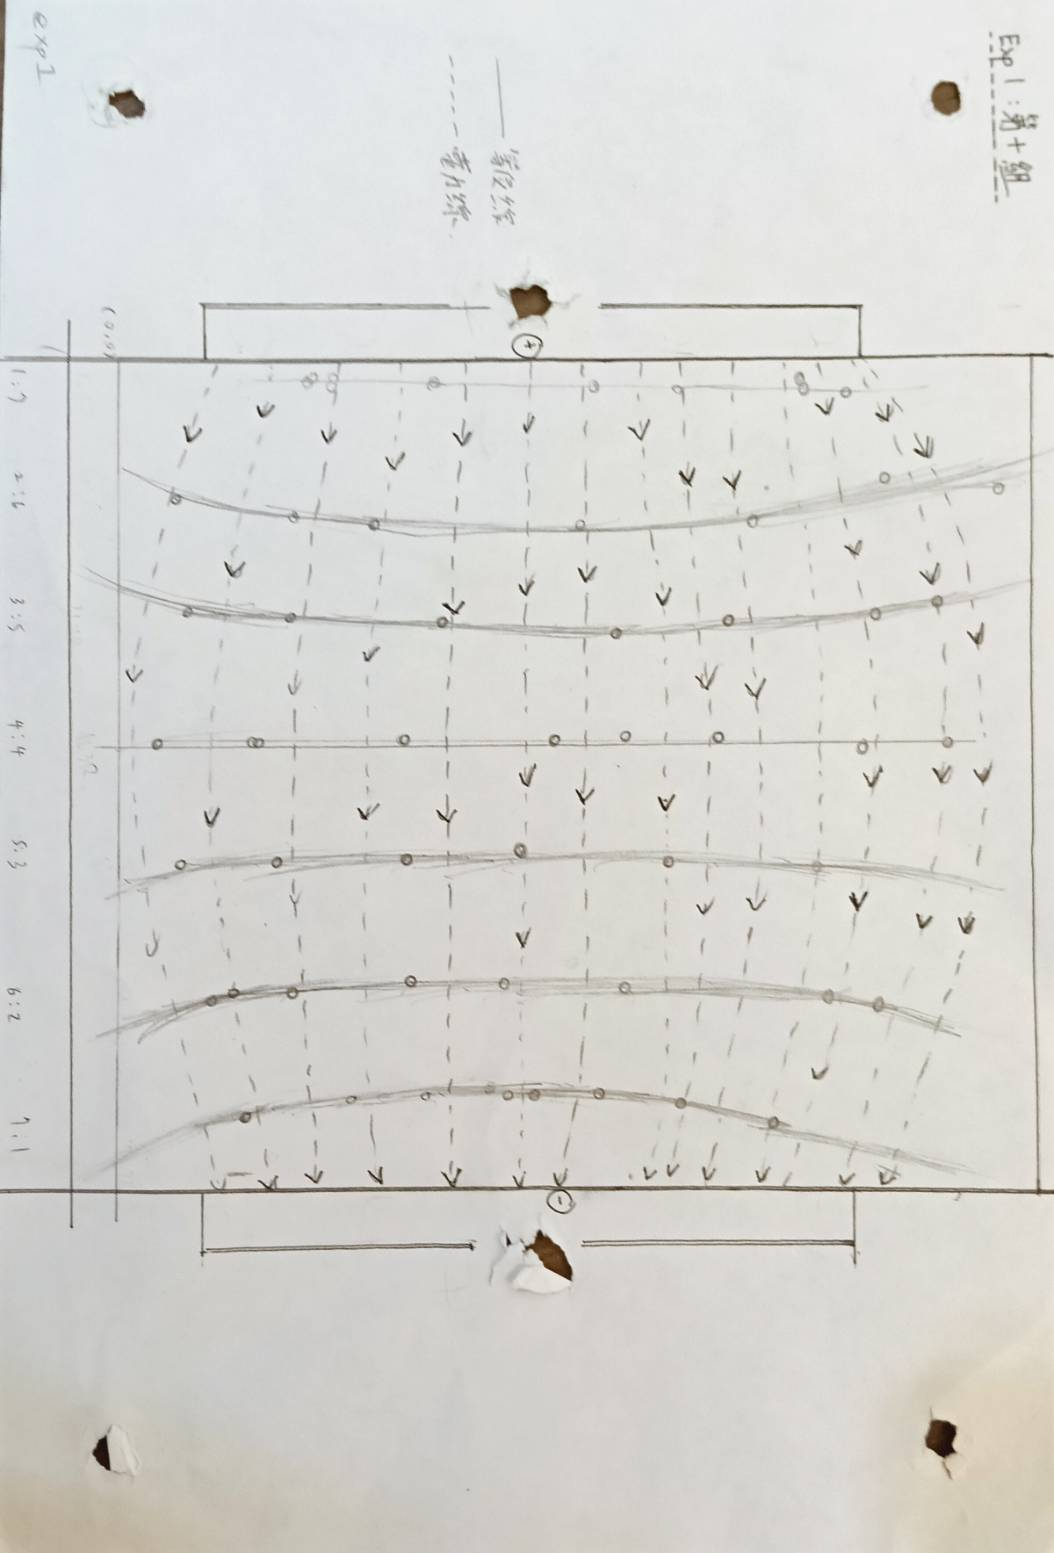
\includegraphics[width=10cm, angle=90]{graph/exp1.jpg}
    \caption{實驗結果圖一} 
    \label{fig:exp1}     
\end{figure}

在本實驗中，兩電極平行排列且皆是長方形，所以兩電極等位線圖形相互對稱，在理想情況下，兩電極的垂直平分線上電位疊加後為0。但實際量測後，中央等電位線距離左方電極6.7cm，距離右方電極有7.7cm，兩者並不相等，我們認為可能原因是儀器上的串聯電阻並不是各個都相等，所以我們使用三用電表量測各區間的電阻後，得到下表:
\begin{table}[H]
    \centering
    \caption{不同電位點之電阻值測量結果} % 建議標題稍微擴充更正式
    \label{tab:resistance_data}
    \begin{tabular}{|c|c|}
        \hline
        測量點 & 電阻值 ($M\Omega$) \\ \hline
        $R_1$ & 13.81 \\ \hline
        $R_2$ & 13.89 \\ \hline
        $R_3$ & 13.66 \\ \hline
        $R_4$ & 13.72 \\ \hline
        $R_5$ & 13.52 \\ \hline
        $R_6$ & 13.70 \\ \hline
        $R_7$ & 13.55 \\ \hline
        $R_8$ & 13.77 \\ \hline
    \end{tabular}
\end{table}

由表\ref{tab:resistance_data}，因為串聯電阻值都並不相同，所以檢流計所連結的點位，並非理論上的零等位點，而$R_1 - R_4$電阻值加總大於$R_5 - R_8$，所以才會出現讓原本預期在幾何中心出現的零電位點向左邊偏移。

\subsection{實驗二}

\begin{figure}[H] 
    \centering    
    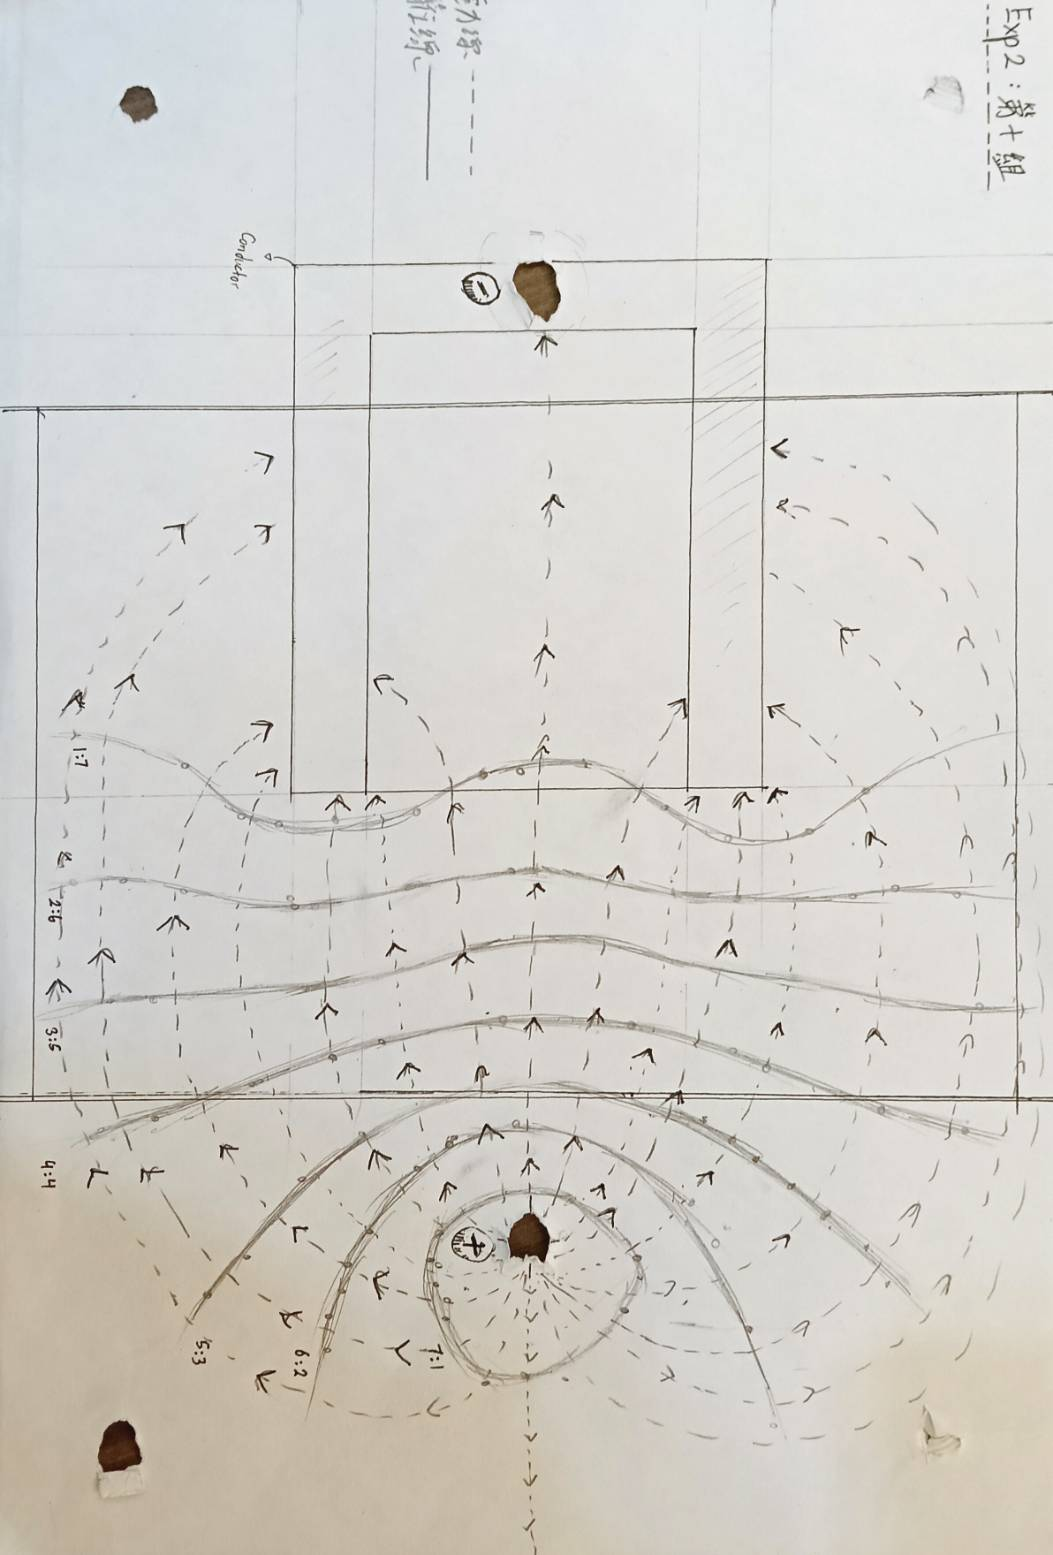
\includegraphics[width=10cm, angle=90]{graph/exp2.jpg}
    \caption{實驗結果圖二} 
    \label{fig:exp2}     
\end{figure}
在實驗二中，左方為U字形電極，雖說導體內部電場應為0，但因為U字形電極並非完全封閉，而是有一個開口，使得電力線仍能進入其中，我們也觀察到，電力線大多都指向U字形電極尖端，對應了尖端放電的概念，所以電場強度較大。

\subsection{實驗三}

\begin{figure}[H] 
    \centering    
    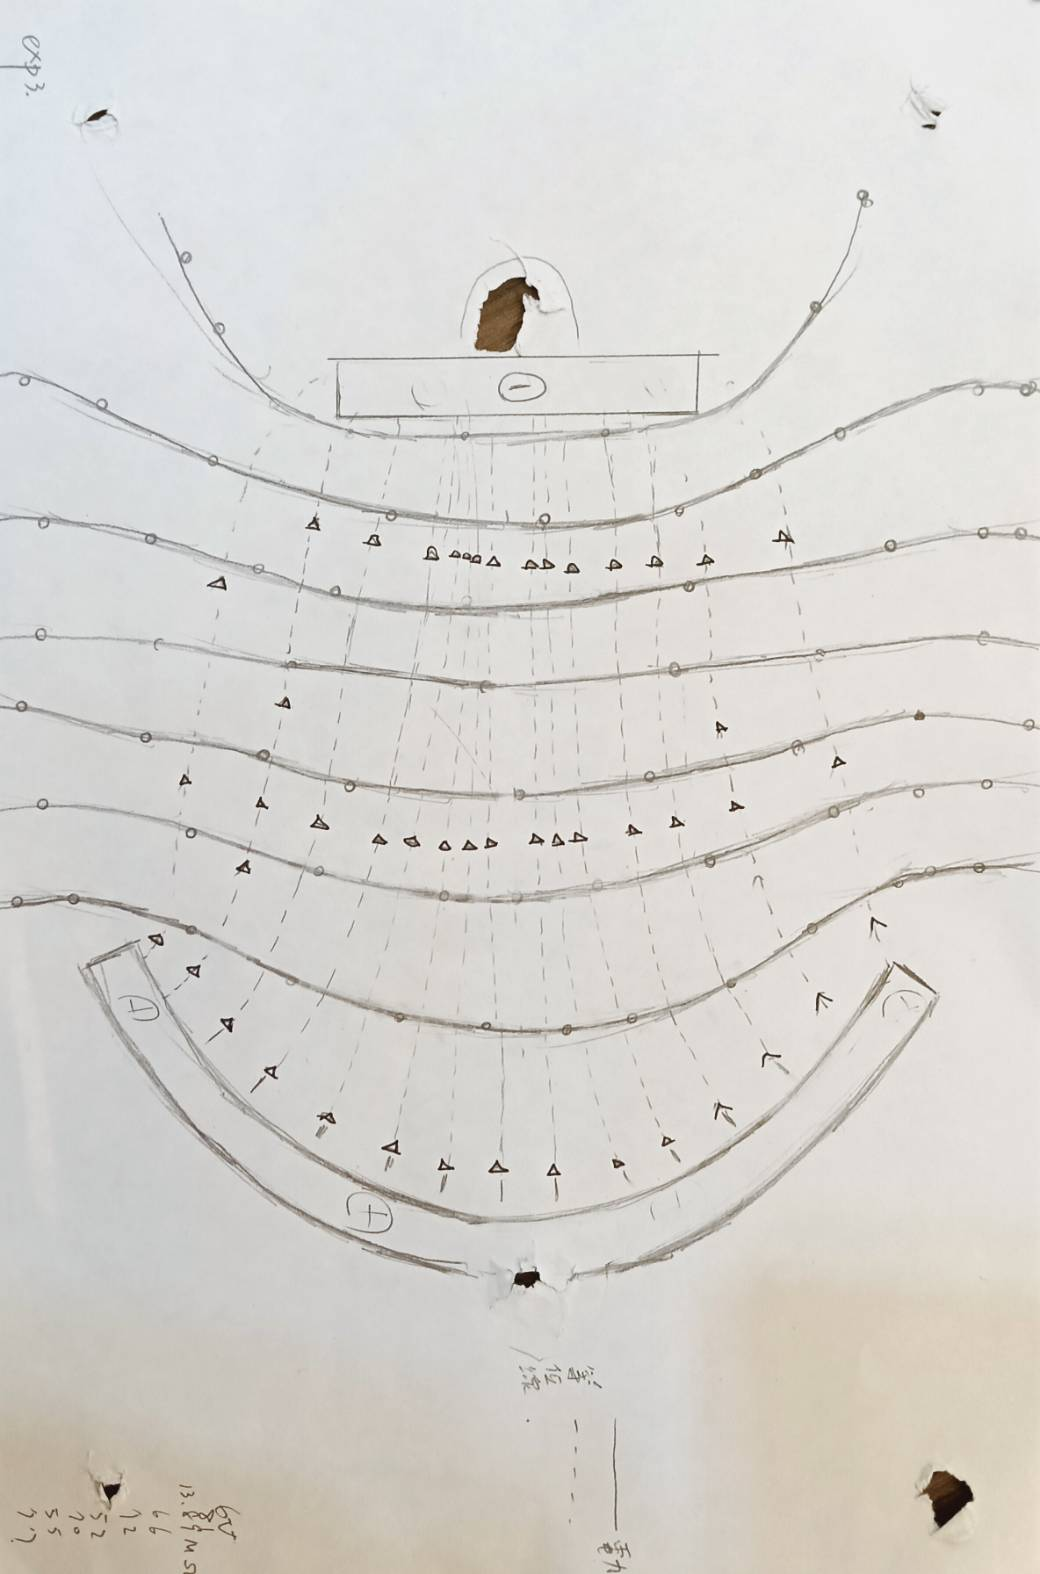
\includegraphics[width=10cm, angle=90]{graph/exp3.jpg}
    \caption{實驗結果圖三} 
    \label{fig:exp3}     
\end{figure}
實驗三中，由於右側半圓形電極的表面積較大，電荷分布較為分散。根據高斯定律與電荷密度公式 $\sigma = \frac{Q}{A}$，在相同電位差下，較大的表面積導致表面電荷密度 $\sigma$ 較低。因此，從該電極發散出的電力線密度較為稀疏，兩等電位線間距也較寬。相對的，左側電極表面積較小，電力線密度也較高，等位線間距也較窄。